\kapitel{Task Definition}
\thispagestyle{plain}
\renewcommand\section{\stdsection}

\sectionroman{Einführung}
Es werden vermehrt Cyberangriffe publik, wo Schadcode im Einsatz ist, welcher sich nicht nur auf einem infizierten System niederlässt, sondern weitere Systeme im Netz befällt. Das Ziel oder Resultat ist dabei oft die komplette Infiltrierung einer Organisation. In der Analyse solcher Fälle sind Information und Zeit ein Schlüssel zum Erfolg. Folglich ist die Bereitschaft "Readiness" für ein solches Ereignis ein entscheidender Faktor.

\sectionroman{Aufgabe}
Ziel dieser Arbeit ist es, ein Tool zu erstellen, welches die Bewertung der eigene Readiness erlaubt aber auch im Analysefall eine Unterstützung bietet. Readiness betrifft viele Aspekte und einfache Dinge wie korrekte Zeitstempel in Logs, deren Vollständigkeit oder die Bereitstellung von Backups. In der konkreten Aufgabenstellung soll die Readiness-Analyse primär für Windows-Infrastrukturen anhand von Logs und spezifischen Events erfolgen. Unter anderem soll auf den neusten Publikationen des japanischen Computer Emergency Response Teams (JPCERT/CC) und der öffentlichen Datenbank der MITRE Corporation, dem Adversarial Tactics, Techniques, and Common Knowledge (ATT\&CK™) Wissenspool, basiert werden. Das JPCERT und MITRE haben dabei die Werkzeuge und das generelle Vorgehen von Angreifern analysiert und geben Hinweise, welche Events auf eine mögliche Verseuchung hinweisen.

\subsectionroman{Abgrenzung}
Es geht nicht darum neue Angriffsvektoren zu finden.

\subsectionroman{Tätigkeiten}
\begin{itemize}
    \item Projektmanagement und Dokumentation
    \item Einarbeitung in Incident Handling und Forensik
    \item Einarbeitung in Angriffstechniken und Werkzeuge
    \item Einarbeitung in Abwehrtechniken und Härtung von Systemen
    \item Studium öffentlicher Quellen und verfügbaren Tools
    \item Umsetzung eines Analyzers gemäss Anforderungen basierend auf etablierten Frameworks    
\end{itemize}

\sectionroman{Vorgehen}
Im Rahmen der allgemeinen Richtlinien zur Durchführung von Studien- und Bachelorarbeiten gemäss eigenem Projektmanagementplan. Dieser Projektmanagementplan ist als Erstes zu erstellen und enthält insbesondere:
\begin{itemize}
    \item Die Beschreibung des dem Projektcharakter angepassten Vorgehensmodells.
    \item Eine erste Aufteilung der Aufgabe in gemeinsam und einzeln zu bearbeitende Teile unter Berücksichtigung der vorgegebenen Teilaspekte. Die genaue Aufteilung muss spätestens nach der Technologiestudie (Elaboration) erfolgen.
    \item Den Projektplan (Zeitplan) und die Meilensteine.
\end{itemize}

\sectionroman{Anforderungen}
Es geht primär darum einen Analyzer zu erstellen um die "Readiness for Tailored Attacks and Lateral Movement Detection" beurteilen zu können. Idealerweise kann dieses Tool von einem IT Administrator ohne spezielle Kenntnisse und grossartige Installationsprozeder ausgeführt werden. 
\\\\
Schematisch aber nicht bindend werden folgende Schritte auszuführen sein
\begin{itemize}
    \item Definition der Requirements für einen neuen/verbesserten Analyzer
    \item Design und Analyse basierend auf den Vorgaben
    \item Vorschläge für die Umsetzung oder Verbesserung eines 
    \begin{itemize}
        \item Readiness Analyzers
        \item Readiness Optimizers
        \item Compromise Analyzers
    \end{itemize}
    \item Implementation der Funktionalität und Erstellung eines Benutzerhandbuch
    \item Erweiterung der Analyzer um neue Erkenntnisse, Werkzeuge und Indicators
    \item Dokumentation der Software und Skripte
\end{itemize}

\subsectionroman{Technologien}
\begin{itemize}
    \item Windows Workstations, Windows Server, Windows Security generell
    \item Windows Event Logs, Security und Audit Logs
    \item Windows On-Board Tools, Sysinternals Toolkit
    \item Active Directory Service (AD) Services
    \item Group Policy Objects (GPO)
    \item PowerShell, .NET, Python, Windows Batch
\end{itemize}

\sectionroman{Infrastruktur}
Die Arbeiten werden auf den Rechnern der Studenten durchgeführt. Zusätzlich benötigte Software oder Hardware wird bei Bedarf und nach Rücksprache mit Compass Security zur Verfügung gestellt. 

\sectionroman{Erwartete Resultate}
\subsectionroman{In elektronischer Form}
\begin{itemize}
    \item lauffähiges Toolkit und kompletter Source Code
    \item komplette Software Dokumentation (Use Cases, Klassenmodell, Sequenzdiagramme usw. in UML)
    \item komplette Use Cases und Erfolgs-Szenarien resp. Musterlösungen
    \item alle Dokumente und Protokolle (vorzugsweise in englischer Sprache)
\end{itemize}

\subsectionroman{Auf Papier}
Gemäss der Anleitung der HSR: \url{\\\\hsr.ch\\root\\alg\\skripte\\Informatik\\Fachbereich\\Studienarbeit_Informatik}
Es muss aus den abgegebenen Dokumenten klar hervorgehen, wer für welchen Teil der Arbeit und der Dokumentation verantwortlich war (detaillierte Zeiterfassung).

\sectionroman{Termine}
Termine gemäss der HSR: \url{\\\\hsr.ch\\root\\alg\\skripte\\Informatik\\Fachbereich\\Studienarbeit_Informatik\\SAI\\Termine}

\begin{table}[H]
    \centering
    \begin{tabular}{| p{2.5cm} | p{13.5cm} |}\hline
        \textbf{Datum} & \textbf{Task}  \\ \hline
        17.09.2018 & Beginn der Arbeit, Ausgabe der Aufgabenstellung durch den Betreuer. \\ \hline  
        18.12.2018 & Erfassung des Abstracts im Online-Tool \url{https://abstract.hsr.ch/} Die Studierenden geben den Abstract für die Diplomarbeitsbroschüre zur Kontrolle an ihren Betreuer/Examinator frei.  
        \par\vspace{4mm}
        Der Betreuer/Examinator gibt das Dokument mit dem korrekten und vollständigen Abstract zur Weiterverarbeitung an das Studiengangsekretariat frei 
        \par\vspace{4mm}
        Vorlagen sowie eine ausführliche Anleitung betreffend Dokumentation stehen auf dem Skripteserver zur Verfügung.\\ \hline  
        21.12.2018 & Der Betreuer/Examinator gibt das Dokument mit dem korrekten und vollständigen Abstract der Broschüre zur Weiterverarbeitung an das Studiengangsekretariat frei.
        \par\vspace{4mm}
        Hochladen aller verlangten Dokumente auf \url{archiv-i.hsr.ch} Abgabe des Berichts an den Betreuer bis 12.00 Uhr \\ \hline      
    \end{tabular}
\end{table}

\subsectionroman{Zeitplan und Meilensteine}
Zeitplan und Meilensteine für das Projekt sind von den Studenten selber zu erarbeiten und zusammen mit dem Projektmanagementplan abzuliefern. Die Meilensteine sind bindend. Der erste Meilenstein ist vorgegeben. Mit den Betreuern werden regelmässige Sitzungen zur Fortschrittskontrolle durchgeführt.

\sectionroman{Betreuung}
Die Arbeiten werden durch Cyrill Brunschwiler betreut. Der Gegenleser ist noch nicht bestimmt.

\subsectionroman{Kontakt}
Cyrill Brunschwiler, Managing Director, Compass Security Schweiz AG\\
Weststrasse 50, 8003 Zürich, Switzerland\\
Werkstrasse 20, 8645 Jona, Switzerland
\\\\
+41 55 214 41 73 \ \\
\href{mailto:cyrill.brunschwiler@compass-security.com}{cyrill.brunschwiler@compass-security.com}\ \\
\href{mailto:cyrill.brunschwiler@hsr.ch }{cyrill.brunschwiler@hsr.ch} \ \\
\url{https://fb.compass-security.com/inbox/hUGXMr2EeZ2V7b}

\sectionroman{Unterschriften}
\begin{figure}[H]
    \centering
    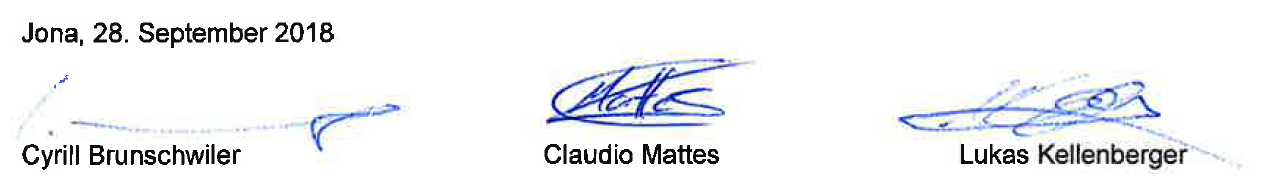
\includegraphics[width=1\linewidth]{assets/task-definition/task_signs.png}
\end{figure}


\renewcommand\section{\clearpage\stdsection}



